\newcommand{\yplus}{\ensuremath{y^+}}
\newcommand{\uplu}{\ensuremath{u^+}}
\section{Boundary layer}
\label{sec:bl}
Three separate separation regions exist on the airfoil: one on the upper surface
close to the leading edge and two on the upper and lower surfaces close to the
trailing edge. The rest of this section is split between those two regions. Moreover,
\Cref{fig:airfoil_sections} shows the various regions as well as locations where
$\yplus,\uplus$ plots were generated.

\begin{figure}
    \centering
    \includegraphics[width=1.0\textwidth]{./figs/airfoil_sections.pdf}
    \caption{Various flow regimes over the airfoil. Profile locations are the locations
        at which \uplu and \yplus are plotted.}\label{fig:airfoil_sections}
\end{figure}

\subsection{Leading edge}
\Cref{fig:cf_upper_le} shows a skin friction distribution zoomed-in close to the leading
edge where $c_f$ drops below zero. Again, $c_f$ is proportional to the velocity gradient
in the normal direction $\partial u/\partial y$ and care was taken in determining the sign
of $c_f$ such that regions of negative $c_f$ may directly be taken as regions of
recirculation. Moreover, \Cref{fig:recirculation_upper} shows
streamlines at that location, clearly illustrating the recirculation bubble in that
same region.

\begin{figure}
    \centering
    \includegraphics[width=1.0\textwidth]{./figs/cf_upper_le.pdf}
    \caption{Skin friction coefficient over the upper airfoil surface zoomed in
        at the recirculation region. Flow separates and reattaches before
        and after recirculation region, respectively.}\label{fig:cf_upper_le}
\end{figure}

\begin{figure}
    \centering
    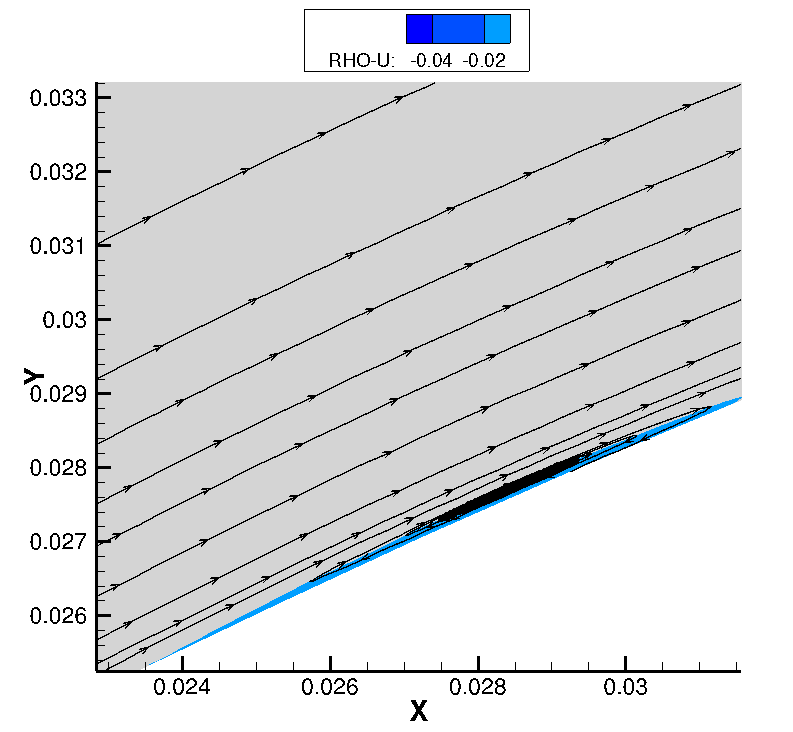
\includegraphics[width=1.0\textwidth]{./figs/recirculation_upper.png}
    \caption{Streamlines over the upper airfoil surface close to and inside the
        recirculation bubble. The blue region corresponds to the recirculation
        bubble.}\label{fig:recirculation_upper}
\end{figure}

One may guess the following scenario. The flow prior to the bubble is laminar, thus has
low momentum close to the wall. Unable
to fight the adverse pressure gradient, flow reversal occurs. This essentially trips
the flow into the turbulent regime. Flow in that regime has a larger $\partial u/\partial y$
near the wall, and thus is able to reattach and climb the pressure hill over most of the
remaining airfoil length until it separates again (see next subsection).
Thus, the fluid would be in the turbulent regime over most of the airfoil!

Of course, this scenario based on a heuristic, however the \uplu plots
will show it to be true! The \uplu and \yplus plots before and after separation
are provided in~\Cref{fig:uplus_upper}. For completeness, the various wall regions are defined
in~\Cref{tab:wallregions}. Let's first discuss the plot after separation and then
before separation.

\begin{table}
    \centering
    \caption{Relevant wall regions and their defining properties~\cite{pope}}\label{tab:wallregions}
    \begin{tabular}{@{}l c p{0.4\textwidth}@{}}
        \toprule
        Region & Location & Defining property\\
        \midrule
        Viscous wall region & $\yplus < 50$ & Viscous contribution to shear stress is significant.\\
        Outer layer & $\yplus > 50$ & Direct effects of viscosity on velocity are negligible. \\
        Viscous sublayer & $\yplus < 5$ & Reynolds shear stress negligible compared to viscous stress.\\
        Buffer layer & $5 < \yplus < 30$ & Region between viscous sublayer and log-law region.\\
        Log-law region & $\yplus > 30, y/\delta < 0.3$ & Log-law holds. Reynolds stress is dominant.\\
        Inner layer & $y/\delta < 0.1 $ & Velocity determined by $u_t$ and \yplus, independently of
            $U_\infty$.\\
        \bottomrule
    \end{tabular}
\end{table}

\subsubsection{After separation}
In the viscous sublayer ($\yplus < 5$) there is good agreement between the MECH 539 curve
and the $\yplus = \uplu$ curve. On the other hand, agreement is not so good in the log-law region
($\yplus > 30$) between the MECH 539 curve and the log-law curve. However, the
MECH 539 curve is approximately linear (on a log scale) in that region. Seeing as how the law of the wall
is universal~\cite{kim}, that large a discrepancy may be attributed to either the solver,
the inherent error that comes with solving the RANS equations, to the post-processing
or a combination of those. In any case, the flow after separation exhibits some turbulence behavior.

\subsubsection{Before separation}
The curve follows the $\yplus = \uplus$ curve until the end of the viscous wall region and then plateaus.
In other words, the effects of the Reynold stress are negligible in the entire inner layer, especially
in the viscous wall region. Hence, the flow can be said to be laminar, since viscous contributions
to shear stress dominate throughout the whole viscous wall region.

\begin{figure}
    \centering
    \includegraphics[width=0.85\textwidth]{./figs/uplus_upper.pdf}
    \caption{Dimensionless velocity profile at various locations. The viscous sublayer, buffer layer and
        log-law regions are separated by grid lines (left to right).}
    \label{fig:uplus_upper}
\end{figure}

\subsection{Trailing edge}
The skin friction coefficient near the trailing edge is shown in~\Cref{fig:cf_te} and streamlines are shown
in~\Cref{fig:recirculation_te}. Again, the recirculation bubble corresponds to the region of negative
$c_f$. Dimensionless velocity profiles before the bubble (on both surfaces) are shown in~\Cref{fig:uplus_te}.
Similar to the reasoning above, it can be said that flow on the upper surface is turbulent and flow
on the lower surface is laminar.

\begin{figure}
    \centering
    \includegraphics[width=\textwidth]{./figs/cf_te.pdf}
    \caption{Skin friction coefficient near the trailing edge for the upper surface (top) and
        lower surface (bottom).}\label{fig:cf_te}
\end{figure}

\begin{figure}
    \centering
    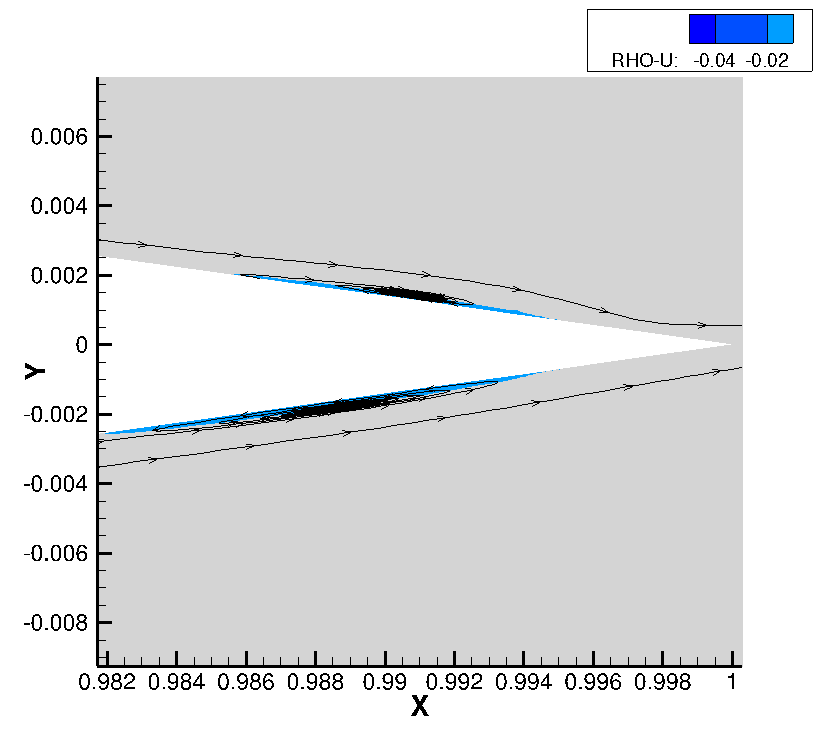
\includegraphics[width=1.0\textwidth]{./figs/recirculation_te.png}
    \caption{Streamlines on upper and lower surface near trailing edge.}\label{fig:recirculation_te}
\end{figure}

\begin{figure}
    \centering
    \includegraphics[width=0.85\textwidth]{./figs/uplus_te.pdf}
    \caption{Dimensionless velocity profile close to trailing edge before recirculation zones.}
    \label{fig:uplus_te}
\end{figure}
